\begin{frame}
\frametitle{La Edad}

\begin{center}
\Huge{21 años}
\end{center}
\end{frame}

\begin{frame}
\frametitle{El Año}

\begin{center}
\Huge{2017}
\end{center}
\end{frame}

\begin{frame}
\frametitle{La Gente -- Ottawa, mayo 2017}
\begin{center}

\includegraphics[width=\textwidth]{devmeet-2017.jpg}
\end{center}
\end{frame}

\begin{frame}
\frametitle{El Código}

\begin{itemize}
\item Replicación Lógica
\item Ejecución en paralelo
\item Particionamiento declarativo
\item CREATE STATISTICS
\item Quórum de commits
\item Autentificación SCRAM
\item Mejorada implementación del ejecutor
\item WAL para índices hash
\item XMLTABLE

\end{itemize}
\end{frame}

\begin{frame}[fragile]
\frametitle{Replicación Lógica}

\begin{lstlisting}
CREATE PUBLICATION publicacion
         FOR TABLE usuarios, clientes;
\end{lstlisting}
\pause

\begin{lstlisting}
CREATE SUBSCRIPTION suscripcion
         CONNECTION 'host=el_remoto dbname=usuarios ...'
        PUBLICATION publicacion;
\end{lstlisting}
\end{frame}

\begin{frame}[fragile]
\frametitle{Ejecución de consultas en paralelo (múltiples CPUs)}

\footnotesize
\begin{lstlisting}
                      QUERY PLAN
-------------------------------------------------------------------------------
Finalize Aggregate
 -> Gather
    Workers Planned: 2
    -> Partial Aggregate
       -> Merge Join
          Merge Cond: (enorme.col1 = grande.col1)
          -> Sort
             Sort Key: enorme.col1
             -> Parallel Bitmap Heap Scan on enorme
                Recheck Cond: ((col1 >= '100000'::numeric) 
                -> Bitmap Index Scan on idx1_enorme 
                   Index Cond: ((col1 >= '100000'::numeric) 
          -> Parallel Index Only Scan using idx1_grande on grande
             Index Cond: ((col1 >= '1000'::numeric)

\end{lstlisting}
\end{frame}

\begin{frame}[fragile]
\frametitle{Particionamiento de verdad}

\footnotesize
\begin{lstlisting}
CREATE TABLE facturas (id INTEGER NOT NULL,
                          fecha_emitida DATE, monto_total NUMERIC /*, ... */)
PARTITION BY RANGE (fecha_emitida);
\end{lstlisting}

\pause
\begin{lstlisting}
CREATE TABLE facturas_2017
   PARTITION OF facturas
    FOR VALUES FROM ('2017-01-01') TO ('2018-01-01');
\end{lstlisting}
\end{frame}

\begin{frame}[fragile]
\frametitle{\texttt{CREATE STATISTICS}}

\begin{lstlisting}

CREATE STATISTICS cpostal_ciudad (ndistinct)
ON (cod_postal, ciudad) FROM direcciones;

\end{lstlisting}
\end{frame}

\begin{frame}[fragile]
\frametitle{Quorum commit (replicación síncrona)}

\begin{lstlisting}
postgresql.conf:

synchronous_standby_names =
         ANY 2 (buenos_aires, santiago, montevideo)

         FIRST 2 (westminster, oxford,
                   cambridge, gloucester)
\end{lstlisting}
\end{frame}

\begin{frame}[fragile]
\frametitle{Autentificación SCRAM}

\begin{lstlisting}
pg_hba.conf:

    hostssl   all      all      129.95.2.0/24     SCRAM-SHA-256

postgresql.conf:

    password_encryption = scram-sha-256
\end{lstlisting}
\end{frame}

\begin{frame}[fragile]
\frametitle{Nuevo ejecutor: evaluador de expresiones}

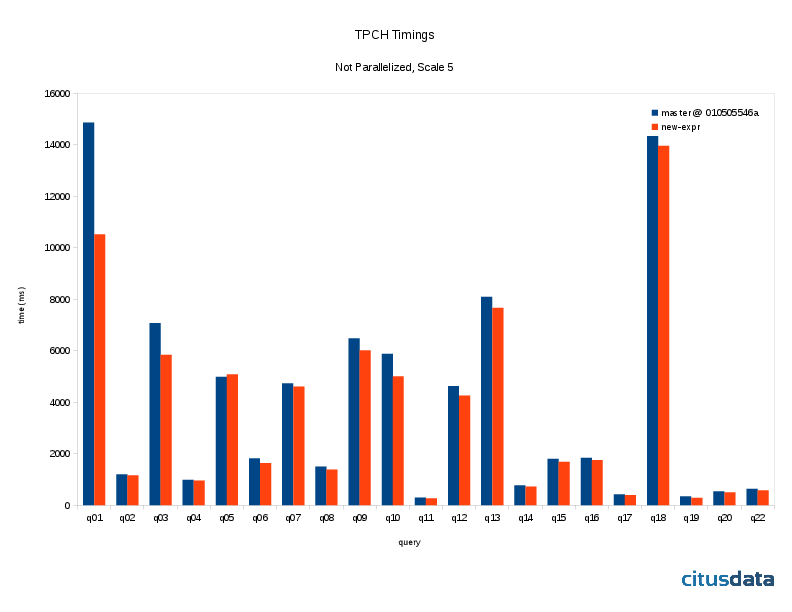
\includegraphics[width=0.95\textwidth]{exec.png}
\end{frame}

\begin{frame}[fragile]
\frametitle{WAL para índices \texttt{hash}}

\begin{lstlisting}
CREATE INDEX idxhash ON tabla USING hash ( columnas );
\end{lstlisting}
\end{frame}

\begin{frame}[fragile]
\frametitle{\texttt{XMLTABLE}}
\footnotesize
\begin{lstlisting}
SELECT xmltable.*
  FROM hoteldata,
       XMLTABLE ('/hotels/hotel/rooms/room' PASSING hotels
                 COLUMNS
                    id FOR ORDINALITY,
                    hotel_name text PATH '../../name' NOT NULL,
                    room_id int PATH '@id' NOT NULL,
                    capacity int,
                    comment text PATH 'comment' DEFAULT 'A regular room'
                );
\end{lstlisting}
\end{frame}
